\begin{center}
\makeatletter
\@ifundefined{color@atlasink}{\definecolor{atlasink}{HTML}{33312E}}{}
\@ifundefined{color@atlasgray}{\definecolor{atlasgray}{HTML}{9A958C}}{}
\@ifundefined{color@atlasblue}{\definecolor{atlasblue}{HTML}{2E6F9E}}{}
\@ifundefined{color@atlasgreen}{\definecolor{atlasgreen}{HTML}{4C8C3F}}{}
\@ifundefined{color@atlasred}{\definecolor{atlasred}{HTML}{C0473B}}{}
\@ifundefined{color@atlasgold}{\definecolor{atlasgold}{HTML}{D69A2A}}{}
\@ifundefined{atlascaption}{%
  \newcommand{\atlascaption}[3]{\shortstack{\footnotesize Figure~#1. \textbf{#2:}\\#3}}%
}{}
\@ifundefined{glowstroke}{%
  \newcommand{\glowstroke}[3]{%
    \draw[#1, line width=1.5pt, line cap=round]
      plot[domain=#2,samples=100,smooth] (\x,{#3});%
  }%
}{}
\makeatother
\tikzset{
  atlas axes/.style={atlasink, line width=0.7pt, line cap=round, ->},
  atlas curve/.style={line width=1.5pt, line cap=round, line join=round},
  dropline/.style={atlasgray, line width=0.6pt, dash pattern=on 2pt off 2pt},
  atlas dot/.style={fill=atlasink, draw=white, line width=0.4pt, circle, inner sep=0pt, minimum size=4.2pt},
}

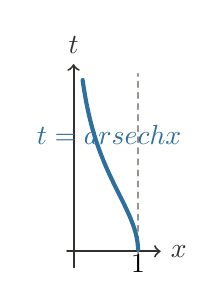
\begin{tikzpicture}[scale=0.82, line cap=round, line join=round]
  \draw[atlas axes] (-0.1,0)--(1.35,0) node[right] {$x$};
  \draw[atlas axes] (0,-0.25)--(0,2.9) node[above] {$t$};
  \draw[dropline] (1,-0.2)--(1,2.75);
  \glowstroke{atlasblue}{0.14:1}{ln(1/\x+sqrt(1/(\x*\x)-1))}
  \fill[atlas dot] (1,0) node[below] {$1$};
  \node[atlasblue] at (0.55,1.8) {$t=\operatorname{arsech}x$};
\end{tikzpicture}

\atlascaption{HI5}{Inverse hyperbolic secant}{Domain $(0,1]$ and range $[0,\infty)$; the inverse uses the nonnegative branch of $\operatorname{sech}$.}
\end{center}


\begin{definitionbox}{Definition}
\begin{definition}[Inverse hyperbolic secant]
\label{def:inverse-hyperbolic-secant}
The \emph{inverse hyperbolic secant} function is the inverse of
$\operatorname{sech}$ after $\operatorname{sech}$ is restricted to
$[0,\infty)$. It is denoted by $\operatorname{arsech}$ and has domain
$(0,1]$ and range $[0,\infty)$.
\[
  \operatorname{arsech} x=t
  \quad\Longleftrightarrow\quad
  \operatorname{sech} t=x
  \quad\text{and}\quad
  t\geq 0.
\]
\end{definition}
\end{definitionbox}
\begin{remark*}[Domain and range]
The regular function $\operatorname{sech}:\mathbb{R}\to(0,1]$ is even, so it
is not one-to-one on all of $\mathbb{R}$. The principal inverse uses the
nonnegative branch, where $\operatorname{sech}$ decreases from $1$ toward
$0$ without attaining $0$.
\end{remark*}
\begin{dependencies}
\begin{itemize}
  \item \hyperref[def:hyperbolic-secant]{Hyperbolic secant}
\end{itemize}
\end{dependencies}

\begin{theorembox}{Theorem}
\begin{theorem}[Principal inverse hyperbolic secant identities]
\label{thm:inverse-hyperbolic-secant-identities}
For every $x\in(0,1]$,
\[
  \operatorname{sech}(\operatorname{arsech} x)=x.
\]
For every $t\in[0,\infty)$,
\[
  \operatorname{arsech}(\operatorname{sech} t)=t.
\]
\end{theorem}
\end{theorembox}
\begin{remark*}[Proof]
These are the cancellation laws for the inverse of the restricted function
$\operatorname{sech}|_{[0,\infty)}:[0,\infty)\to(0,1]$.
\end{remark*}
\begin{dependencies}
\begin{itemize}
  \item \hyperref[def:inverse-hyperbolic-secant]{Inverse hyperbolic secant}
\end{itemize}
\end{dependencies}
